\documentclass[tikz, border=10pt]{standalone}
\usepackage{tikz}
\begin{document}
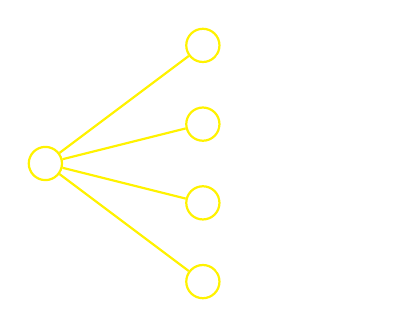
\begin{tikzpicture}[shorten >=0pt, draw=yellow, thick, every node/.style={text=yellow},  xscale=.5, yscale=1 ] 
    \tikzstyle{neuron}=[circle, minimum size=12pt, draw=yellow, thick, fill=none]  % Circles with yellow boundary
    \tikzstyle{input neuron}=[neuron];
    \tikzstyle{hidden neuron}=[neuron];
    \tikzstyle{output neuron}=[neuron];
    \tikzstyle{annot} = [text width=4em, text centered]

    % Input layer
    \node[input neuron] (I) at (0,-2.5) {};

    % Hidden layer
    \node[hidden neuron] (H-1) at (4,-1) {};  
    \node[hidden neuron] (H-2) at (4,-2) {};  
    \node[hidden neuron] (H-3) at (4,-3) {};  
    \node[hidden neuron] (H-4) at (4,-4) {};  

    % Output layer
    \node[output neuron, draw=white] (O) at (8,-2.5) {}; 
    
    % Connect input layer to hidden layer
    \draw (I) -- (H-1);
    \draw (I) -- (H-2);
    \draw (I) -- (H-3);
    \draw (I) -- (H-4);


    % Connect hidden layer to output layer
    \draw [draw=white] (H-1) -- (O);
    \draw [draw=white] (H-2) -- (O);
    \draw [draw=white] (H-3) -- (O);
    \draw [draw=white] (H-4) -- (O);

\end{tikzpicture}
\end{document}

